% c10 —— §4.2 作为 Lagrangian 微扰论的 Feynman 图；§4.3 与模空间相交理论的关系（原书 p.68–75）
% 负责：trans-e

% ===== 原书 p.68 =====
此时，两个顶点$(i,j),(i',j')$对应的$P$的分量不为$0$，只在如上图那样箭头与颜色的组合无矛盾地相接时才出现。此时，若定义这个图$G_{ij}$的权为
\[
w(G_{ij})=\frac{2}{\lambda_i+\lambda_j},
\]
则它与前述着色版本的权一致。设$I=(i_1,\dots,i_k)$，$J=(j_1,\dots,j_k)$。

\begin{center}
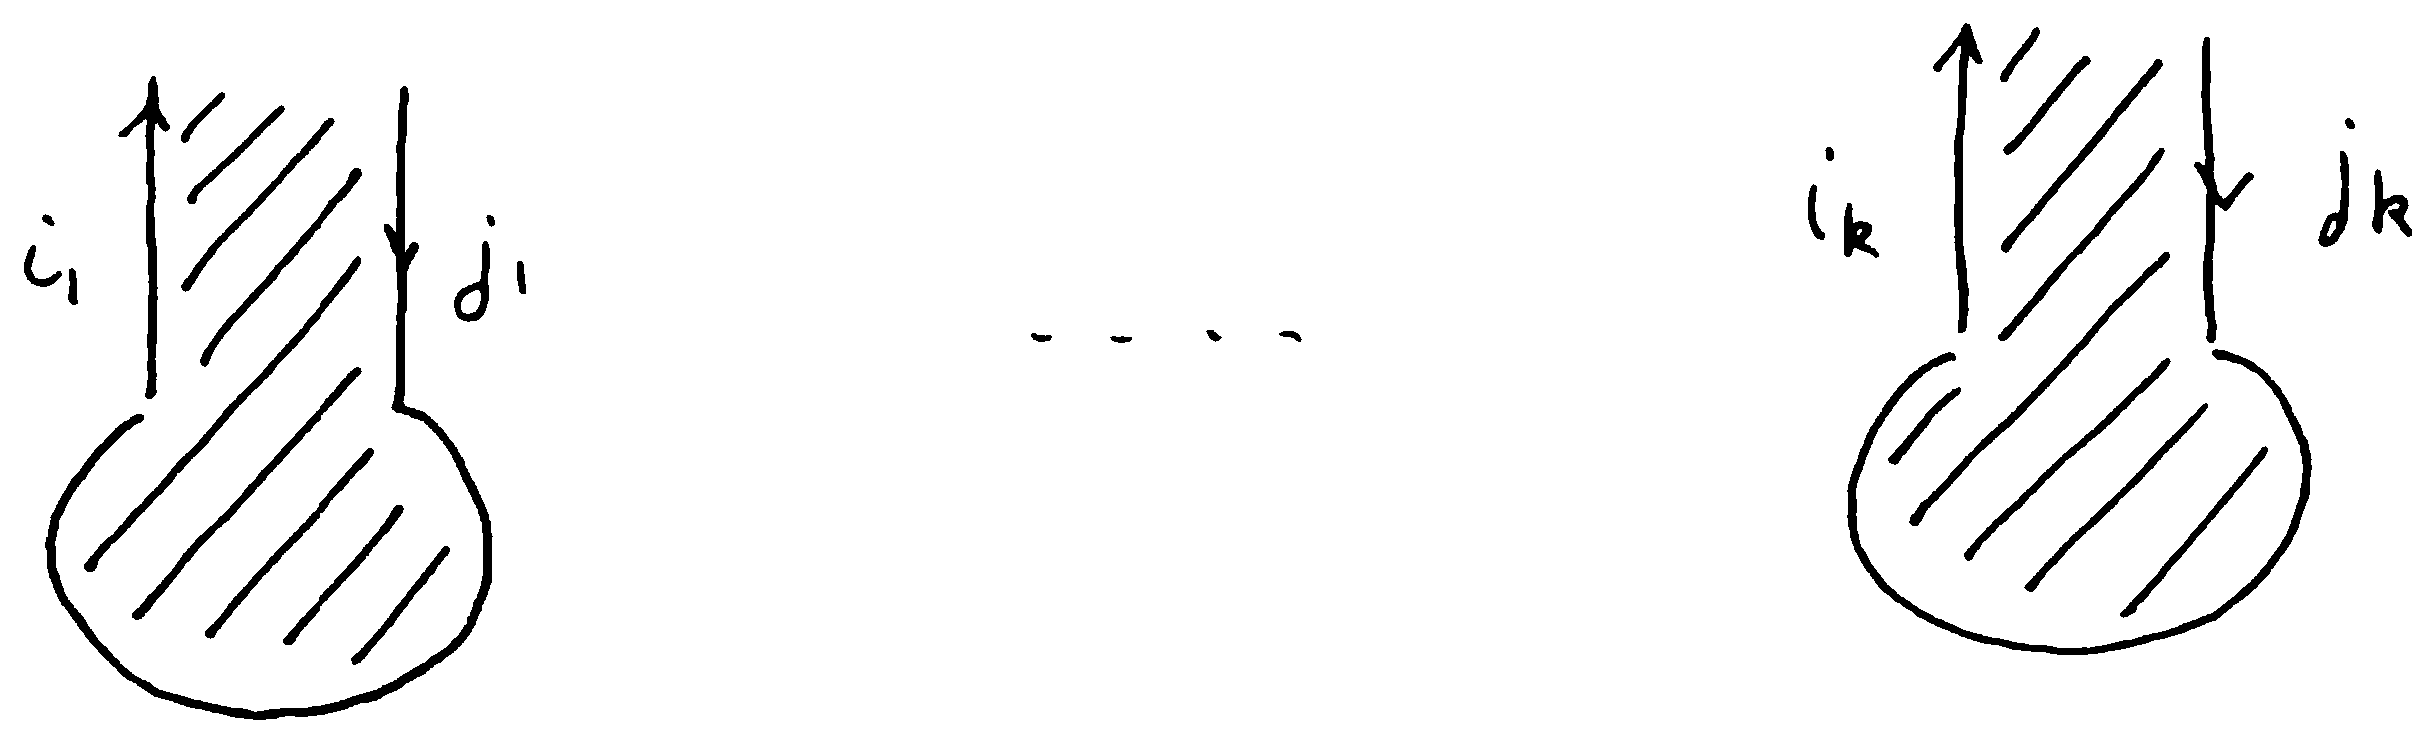
\includegraphics[width=0.56\linewidth]{fig_p74_a.png}
\end{center}

令
\[
\mathcal{A}(I,J)=\{\text{如上所述把 unit 两个一组无矛盾地组合起来所得的图形的全体}\},
\]
并对$\Gamma\in\mathcal{A}(I,J)$定义$w(T)=\prod_{e\in\Gamma}w(e)$。这里$e$是$\Gamma$的边，$w(e)$是先定义好的权。

\transnote{上式左端原书印作$w(T)$，而下文讨论的对象是$\Gamma$，$T$疑为$\Gamma$的排印之误。译本照原文印出。}

\begin{theorem}
\[
\frac{\langle x_{IJ}\rangle}{\langle 1\rangle}
=\sum_{\Gamma\in\mathcal{A}(I,J)}w(\Gamma).
\]
\end{theorem}

\subsection{Lagrangian 微扰论及其 Feynman 图}

以下暂且不论积分的收敛性。对充分小的$t$，把
\[
\langle\exp(tx^3/6)\rangle=\int\exp\Bigl(-\frac{\kappa}{2}x^2+\frac{t}{6}x^3\Bigr)\,dx
\]
按$t$展开，得$\sum_{i=0}^{\infty}\langle\frac{x^{3m}}{6^m m!}\rangle t^m$。把这个系数与三价图

\transnote{上式求和号下标原书印作$i=0$，而被求和的项中出现的指标是$m$，$i$疑为$m$的排印之误。译本照原文印出。}

% ===== 原书 p.69 =====
联系起来数吧。现在固定满足$2e=3v$的自然数$e,v$。
\[
\begin{aligned}
&\#\{\text{边、顶点都已编号，边数 $=e$、顶点数 $=v$ 的三价图}\}\times6^v\\
&\quad=\#\{\text{边、顶点都已编号，且从各顶点伸出的边再标上 $1\sim3$ 的号，}\\
&\qquad\qquad\text{边数 $=e$、顶点数 $=v$ 的三价图}\}\\
&\quad=\#\{\text{把 $(i,1)\sim(1,3)$（$i=1,\dots,v$）这 $3v$ 个顶点两个一组不剩余地}\\
&\qquad\qquad\text{配对的配法}\}\times e!\\
&\quad=e!\,\frac{\langle x^{3v}\rangle}{\langle 1\rangle}\kappa^e
\end{aligned}
\]
这从上一节可以明白。

\transnote{上式中第三行的$(1,3)$依前后文与所附图形应作$(i,3)$，原书如此印出，译本照印。}

现在，对边与顶点都已编号的三价图$\Gamma$，把$\Aut(\Gamma)$定义为边、顶点的编号所成集合的自同构中保持图的连接方式不变者。此时，把$\Gamma$去掉编号后所得者记作$\mathrm{Supp}(\Gamma)$。固定$\mathrm{Supp}(\Gamma)$时，编号的替换有$e!v!$种。在编号的替换中把彼此可由$\Aut(\Gamma)$互相转移者视为同一，则编号了的三价图$\Gamma'$中满足$\mathrm{Supp}(\Gamma')$与$\mathrm{Supp}(\Gamma)$相同者的个数为$\dfrac{e!v!}{\Aut(\Gamma)}$。因此，令
\[
G_{e,v}=\{\Gamma\mid\text{边数 $=e$、顶点数 $=v$ 的三价图}\}
\]
则
\[
\sum_{\Gamma\in G_{e,v}}\frac{e!v!}{\Aut(\Gamma)}6^v
=e!\,\frac{\langle x^{3v}\rangle}{\langle 1\rangle}\kappa^e
\]
成立。因此
\[
\frac{\langle\exp(tx^3/6)\rangle}{\langle 1\rangle}
=\sum_{m=0}^{\infty}\sum_{\Gamma\in G_{e,m}}
\frac{\kappa^{-\frac32 m}}{\Aut(\Gamma)}t^m
\]
成立。进而考虑把$\Gamma$分解为连通分支。把$\Gamma$作为三价图写成
\[
\Gamma=(\Gamma_1^{(1)}\sqcup\cdots\sqcup\Gamma_{m_1}^{(1)})
\sqcup\cdots\sqcup
(\Gamma_1^{(s)}\sqcup\cdots\sqcup\Gamma_{m_s}^{(s)})
\]

% ===== 原书 p.70 =====
即分解为连通分支。这里$\Gamma_j^{(i)}$（$j=1,\dots,m_i$）是彼此同型的三价图，上述分解是按同型者归并的分组。此时
\[
\#\Aut(\Gamma)
=m_1!\cdots m_s!\#\Aut(\Gamma_1^{(1)})\cdots\#\Aut(\Gamma_1^{(s)})
\]
成立，故上式成为
\[
\prod_{\Gamma:\ \text{连通}}
\Bigl(\sum_{m=0}^{\infty}\Bigl(\frac{1}{\Aut(\Gamma)}\Bigr)^m
\frac{1}{m!}(\kappa^{-\frac32}t)^{m v(\Gamma)}\Bigr)
\]
成立。这里$v(\Gamma)$是$\Gamma$的顶点数。因此对两边取对数，得
\[
\log\Bigl(\frac{\langle\exp(tx^3/6)\rangle}{\langle 1\rangle}\Bigr)
=\sum_{\Gamma:\ \text{连通}}\frac{1}{\Aut(\Gamma)}
(\kappa^{-\frac32}t)^{v(\Gamma)}
\]
这样的等式。这称为关于 Feynman 图的展开。

在矩阵模型的情形也作同样的考察，就出现关于带状图的展开。把$f(X)$取为关于$X\in H_n$的函数，令
\[
\langle f(X)\rangle=\int_{H_n}f(X)\exp\Bigl(-\frac12\tr(\Lambda X^2)\Bigr)\,dX
\]
当$f(X)=\exp\bigl(\frac{t}{3}\tr(X^3)\bigr)$时，试把$\langle f(X)\rangle$关于$t$展开。计算$\langle\frac{1}{3^m m!}(\tr(X^3))^m\rangle$。由于$\tr(X^3)=\sum_{i,j,k}x_{ij}x_{jk}x_{ki}$，有
\[
(\tr(X^3))^m
=\sum_{(i_1,j_1,k_1),\dots,(i_m,j_m,k_m)}
(x_{i_1j_1}x_{j_1k_1}x_{k_1i_1})\cdots(x_{i_mj_m}x_{j_mk_m}x_{k_mi_m}).
\]
于是，对$I=(i_1,j_1,k_1),\dots,(i_m,j_m,k_m)\in\{1,\dots,r\}^{3m}$，记
\[
x_I=(x_{i_1j_1}x_{j_1k_1}x_{k_1i_1})\cdots(x_{i_mj_m}x_{j_mk_m}x_{k_mi_m}).
\]
现在把集合$G_I$定义为
\[
G_I=\{\text{把下方的顶点无矛盾地两个一组配对并贴合所得的图形}\}
\]

\transnote{上式及此后诸式中原书用$r$，而此处矩阵是$n$阶、颜色标号取自$1,\dots,n$；$r$疑沿袭前一节（$r$个变量）的记号，译本照原文印出。}

% ===== 原书 p.71 =====
这样来定义。

\begin{center}
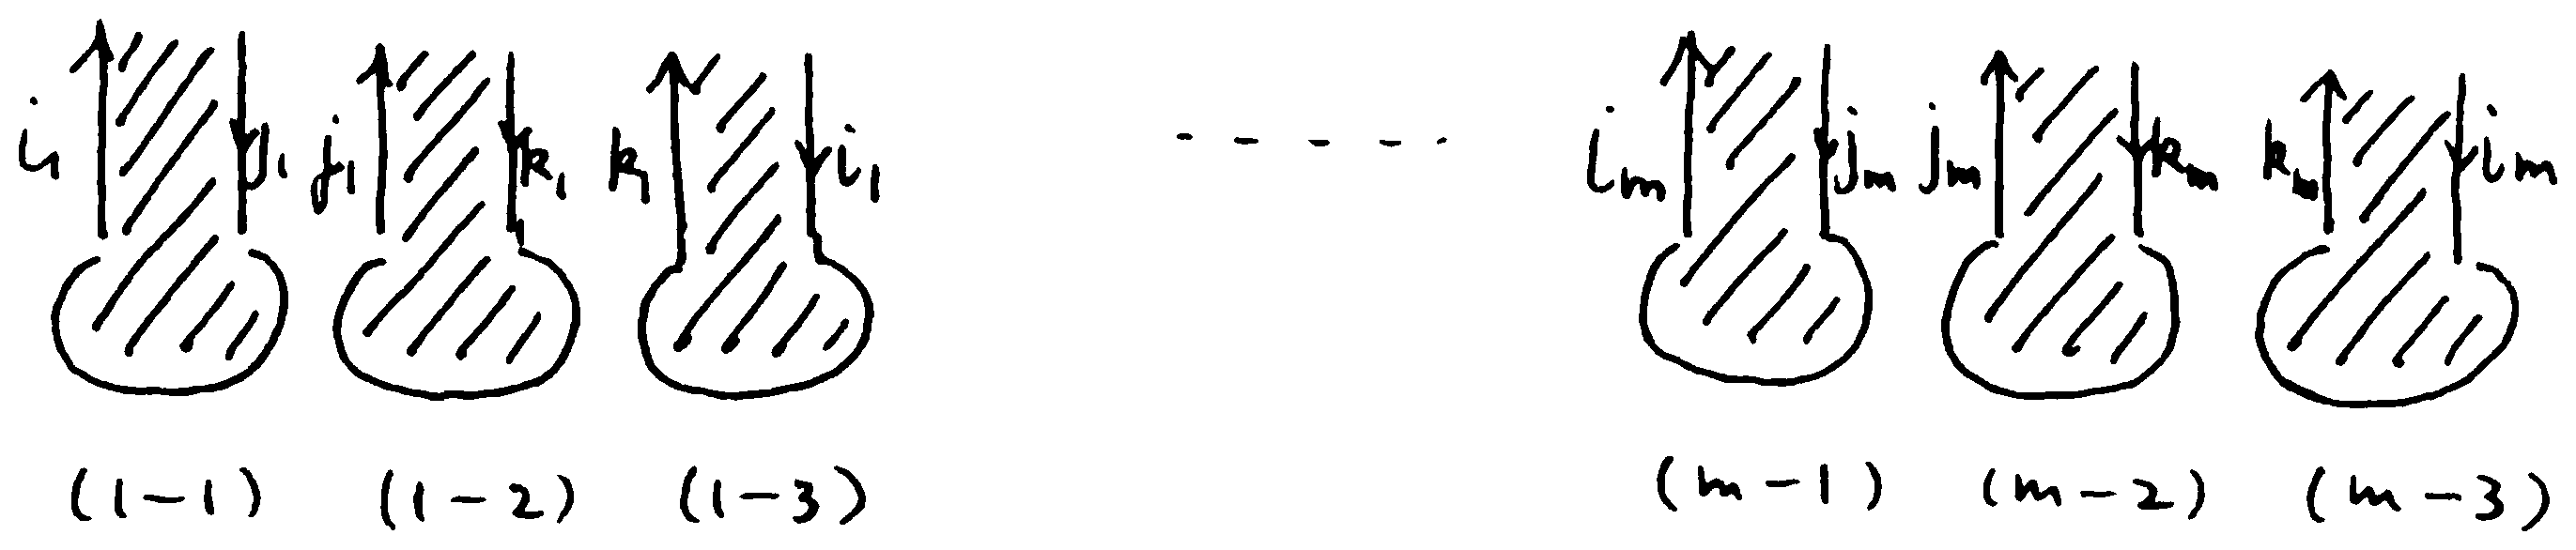
\includegraphics[width=0.80\linewidth]{fig_p77_a.png}
\end{center}

对$\Gamma\in G_I$，把$e\in\Gamma$取为一个组。这个组可看作带有两个边界的短带状图；把$i,j$取为$e$的两个边界上所附的编号，以$\tilde\lambda(e)=\lambda_i+\lambda_j$定义。此时由定理 4.3 得
\[
\frac{\langle x_I\rangle}{\langle 1\rangle}
=\sum_{\Gamma\in G_I}\prod_{e\in\Gamma}\frac{2}{\tilde\lambda(e)}.
\]
接着考虑把$G_I$重新分组。首先，对$\Gamma\in G_I$，如下构成三价带状图。把顶点$(1-1),(2-1),(3-1)$合成一个，考虑下图中那样的「三叉」图。

\transnote{上式中的$(2-1),(3-1)$与图中所附标号$(1-1),(1-2),(1-3)$不符，依文义应作$(1-1),(1-2),(1-3)$。原书如此印出，译本照印。}

\begin{center}
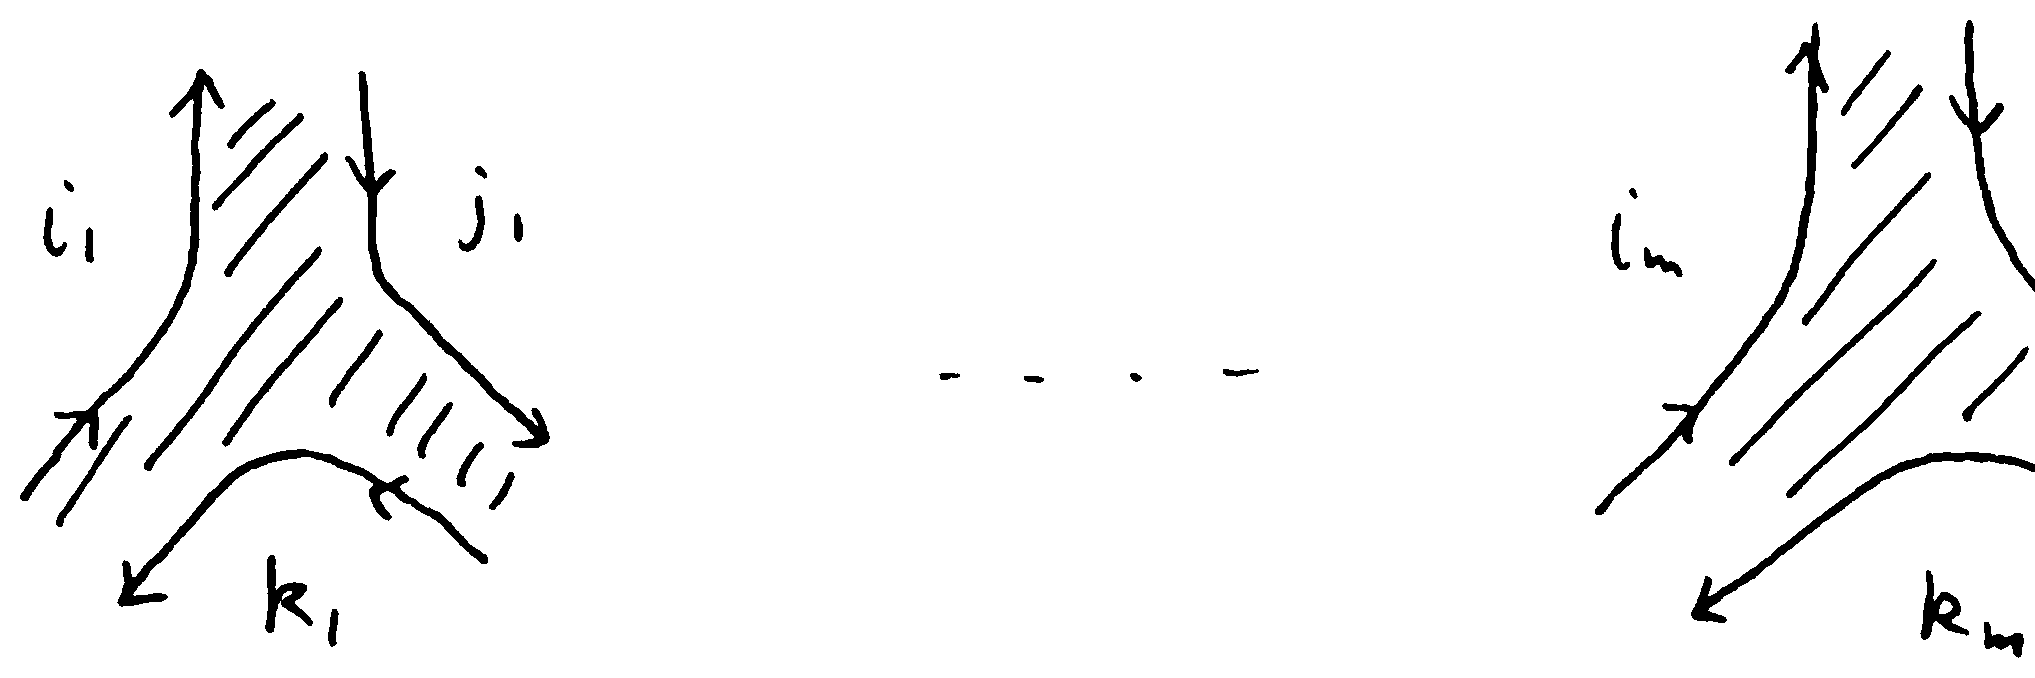
\includegraphics[width=0.78\linewidth]{fig_p77_b.png}
\end{center}

$\Gamma$是把各自的端不剩余且无矛盾地贴合的贴法，故按此把上述带状图贴合。这个带状图带有各顶点的编号与从该顶点伸出的三条边的编号。从一个点伸出的边的编号与给出带状图结构的循环次序相容。此外，边界上标有$1,\dots,r$的颜色。反之，考虑边界带颜色的三价带状图，其上的顶点、边有编号；从一点伸出的三条边的编号与 ribbon structre 相容，取 $1,2,3$。这样的组记为$\tilde\Gamma$。

% ===== 原书 p.72 =====
下面考察它。此时，在边的中点处切开时，就确定出$I=(i_1,j_1,k_1),\dots,(i_m,j_m,k_m)$这样一个$\{1,\dots,r\}^{3m}$的元素。称其为$\tilde\Gamma$的着色。若定义
\[
G_I^\psi=\left\{\begin{array}{l}
\text{边界上标有 $1,\dots,r$ 的颜色，其上的顶点、边的编号，以及从一点伸出的三条边的}\\
\text{ribbon structre 相容的 $1,2,3$ 的编号均已给出，且着色为 $I$ 的三价带状图}
\end{array}\right\},
\]
则忘记边的编号所得的映射$G_I^\psi\to G_I$是$e!:1$的映射。进而定义

\transnote{原文此处的 ribbon structure 印作 ribbon structre，上文（原书 p.71 末行）亦同，译本照原文印出。}
\[
G_\#^c=\left\{\begin{array}{l}
\text{边界上标有 $1,\dots,r$ 的颜色，其上的顶点与边的编号已给出的带状图}
\end{array}\right\},
\]
把$\coprod_IG_I^\psi\to G_\#^c$取为忘记从各顶点伸出的边的次序的映射，则它是$3^v:1$的映射。因此
\[
\begin{aligned}
\frac{\langle(\tr(X^3))^m\rangle}{3^m m!\langle 1\rangle}
&=\frac{1}{3^m m!}\sum_{I\in[1,r]^{3m}}\sum_{\Gamma\in G_I^\psi}
\prod_{e\in\Gamma}\frac{2}{\tilde\lambda(e)}\\
&=\frac{1}{3^m m!e!}\sum_{I\in[1,r]^{3m}}\sum_{\Gamma\in G_I}
\prod_{e\in\Gamma}\frac{2}{\tilde\lambda(e)}\\
&=\frac{1}{m!e!}\sum_{\Gamma\in G_\#^c}\prod_{e\in\Gamma}\frac{2}{\tilde\lambda(e)}
\end{aligned}
\]
成立。对$\Gamma\in G_\#^c$，把$\Aut^c(\Gamma)$定义为$\Gamma$的保持着色的自同构，并令
\[
G^c=\{\text{边界带颜色的带状图，且不考虑顶点、边的编号}\},
\]
则上式写作
\[
\sum_{\Gamma\in G^c}\frac{1}{\Aut^c(\Gamma)}\prod_{e\in\Gamma}\frac{2}{\tilde\lambda(e)}.
\]
现在乘上$t^m$并对$m$求和；为明示$m$，把$G^c,G_\#^c$分别写作$G_m^c,G_{\#,m}^c$。这里$m$是顶点数。

% ===== 原书 p.73 =====
\begin{theorem}
\[
\frac{\langle\exp(\frac{t\tr(X^3)}{3})\rangle}{\langle 1\rangle}
=\sum_{m=0}^{\infty}
\Bigl(\sum_{\Gamma\in G_m^c}\frac{1}{\Aut^c(\Gamma)}
\prod_{e\in\Gamma}\frac{2}{\tilde\lambda(e)}\Bigr)t^m
\]
\end{theorem}

下面考虑把$\Gamma$分解为 connceted component。把$\Gamma$分解为 connceted compoent，并把着色也包含在内按同型者归并，写成

\transnote{本段中原书把 connected 误排为 connceted，把 component 误排为 compoent，译本照原文印出。}

\[
\Gamma=(\Gamma_1^{(1)}\sqcup\cdots\sqcup\Gamma_{m_1}^{(1)})
\sqcup\cdots\sqcup
(\Gamma_1^{(s)}\sqcup\cdots\sqcup\Gamma_{m_s}^{(s)})
\]
则
\[
\Aut^c(\Gamma)=m_1!\cdots m_s!
\#\Aut^c(\Gamma_1^{(1)})^{m_1}\times\cdots\times
\#\Aut^c(\Gamma_1^{(s)})^{m_s},
\]
故令$G_m^{c0}=\{\Gamma\in G_m^c\mid\Gamma\text{ 连通}\}$，得
\[
\begin{aligned}
&\sum_{m=0}^{\infty}\Bigl(\sum_{\Gamma\in G_m^c}\frac{1}{\Aut^c(\Gamma)}
\prod_{e\in\Gamma}\frac{2}{\tilde\lambda(e)}\Bigr)t^m\\
&\quad=\prod_{m=1}^{\infty}\prod_{\Gamma\in G_m^{c0}}
\Bigl(\sum_{k=0}^{\infty}\frac{1}{k!}
\Bigl(\frac{1}{\Aut^c(\Gamma)}\prod_{e\in\Gamma}\frac{2}{\tilde\lambda(e)}\Bigr)^k
t^{km}\Bigr)
\end{aligned}
\]
成立。因此
\[
\log\Bigl(\frac{\langle\exp(\frac{t\tr(X^3)}{3})\rangle}{\langle 1\rangle}\Bigr)
=\sum_{m=1}^{\infty}\sum_{\Gamma\in G_m^{c0}}
\Bigl(\frac{1}{\Aut^c(\Gamma)}\prod_{e\in\Gamma}\frac{2}{\tilde\lambda(e)}\Bigr)t^m
\]
成立。

令$G_{\#m}^{c0}=\{\Gamma\in G_{\#m}^c\mid\Gamma\text{ 连通}\}$，则
\[
\sum_{\Gamma\in G_m^{c0}}\frac{1}{\Aut^c(\Gamma)}
\prod_{e\in\Gamma}\frac{2}{\tilde\lambda(e)}
=\sum_{\Gamma\in G_{\#m}^{c0}}\frac{1}{m!e!}
\prod_{e\in\Gamma}\frac{2}{\tilde\lambda(e)}
\]
成立。进而令
\[
G_{\#m,n}^{b0}=\left\{\begin{array}{l}
\text{带有 $n$ 个已编号的边界、边与顶点均已编号的连通带状图，且顶点数 $=m$}
\end{array}\right\},
\]
\[
G_{m,n}^{b0}=\left\{\begin{array}{l}
\text{带有 $n$ 个已编号的边界的带状图，且顶点数 $=m$}
\end{array}\right\}
\]

% ===== 原书 p.74 =====
并这样来定义。对应边界$1,\dots,n$引入新的变量$u_1,\dots,u_n$，对$\Gamma\in G_{m,n}^{b0}$的边$e\in\Gamma$，以$u_i+u_j$定义$\tilde u(e)$。进而对$J=(j_1,\dots,j_n)\in[1,r]^n$以及$f(u_1,\dots,u_n)\in\C[u_1,\dots,u_n]$，定义$f(u)^J=f(\lambda_{j_1},\dots,\lambda_{j_n})\in\C[\lambda_1,\dots,\lambda_r]$。于是
\[
\begin{aligned}
\sum_{\Gamma\in G_{\#m}^{c0}}\frac{1}{m!e!}
\prod_{e\in\Gamma}\frac{2}{\tilde\lambda(e)}
&=\sum_n\sum_{\Gamma\in G_{\#m,n}^{b0},\ J\in[1,r]^n}
\frac{1}{n!m!e!}\Bigl(\prod_{e\in\Gamma}\frac{2}{\tilde u(e)}\Bigr)^J\\
&=\sum_n\sum_{\Gamma\in G_{m,n}^{b0},\ J\in[1,r]^n}
\frac{1}{n!\Aut(\Gamma)}\Bigl(\prod_{e\in\Gamma}\frac{2}{\tilde u(e)}\Bigr)^J
\end{aligned}
\]
成立。归纳起来，

\begin{theorem}
\[
\log\Bigl(\frac{\langle\exp(\frac{t\tr(X^3)}{3})\rangle}{\langle 1\rangle}\Bigr)
=\sum_{n,m}t^m\sum_{\Gamma\in G_{m,n}^{b0},\ J\in[1,r]^n}
\frac{1}{n!\Aut(\Gamma)}\Bigl(\prod_{e\in\Gamma}\frac{2}{\tilde u(e)}\Bigr)^J
\]
\end{theorem}

\subsection{与模空间相交理论的关系}

把现在的定理与模空间的相交理论合起来思考。type$(g,n)$的三价带状图的顶点数$=-4+4g+2n$，故代入前一章的 main identity
\[
\sum_{d_1+\cdots+d_n=3g-3+n}
\langle\tau_{d_1},\dots,\tau_{d_n}\rangle
\prod_{i=1}^{n}\frac{(2d_i-1)!!}{u_i^{2d_i+1}}
=\sum_{\Gamma\in G_{m,n}^{b0}}\frac{2^{-m}}{\Aut(\Gamma)}
\prod_{e\in\Gamma}\frac{2}{\tilde u(e)}
\]
得
\[
\begin{aligned}
&\log\Bigl(\frac{\langle\exp(\frac{\tr(X^3)}{6})\rangle}{\langle 1\rangle}\Bigr)\\
&\quad=\sum_n\sum_{d_1,\dots,d_n}\langle\tau_{d_1},\dots,\tau_{d_n}\rangle
\sum_{J\in[1,r]^n}\frac{1}{n!}
\Bigl(\prod_{i=1}^{n}\frac{(2d_i-1)!!}{u_i^{2d_i+1}}\Bigr)^J
\end{aligned}
\]
成立。这里约定：当不存在满足$\sum_{i=1}^n d_i=3g-3+n$的$g$时，$\langle\tau_{d_1},\dots,\tau_{d_n}\rangle=0$。

\transnote{上一式的左端（含$\log$的式子），原书印作$\exp(\tr(X^3)/6)$，指数中不含$t$；而定理 4.5 中同一位置印作$\exp(t\tr(X^3)/3)$。此处照原文印出。}

作变量变换
\[
t_d=\sum_{i=1}^{n}\frac{(2d-1)!!}{\lambda_i^{2d+1}},
\]
则上式成为
\[
\begin{aligned}
&\sum_{n=0}^{\infty}\sum_{d_1,\dots,d_n}\frac{1}{n!}
\prod_{i=1}^{n}t_{d_i}\langle\tau_{d_1}\cdots\tau_{d_n}\rangle\\
&\quad=\sum_{m_i\ge0}\frac{1}{m_0!\cdots m_s!}
t_0^{m_0}\cdots t_s^{m_s}\langle\tau_0^{m_0}\cdots\tau_s^{m_s}\rangle
\end{aligned}
\]
而它在形式上可写作
\[
\langle\exp(t_0\tau_0)\exp(t_1\tau_1)\cdots\rangle
=\Bigl\langle\exp\Bigl(\sum_{i\ge0}t_i\tau_i\Bigr)\Bigr\rangle.
\]


% ===== 原书 p.75 =====
\begin{theorem}
在变量变换$t_d=\sum_{i=1}^{n}\frac{(2d-1)!!}{\lambda_i^{2d+1}}$之下，
\[
\log\Bigl(\frac{\langle\exp(\frac{\tr(X^3)}{6})\rangle}{\langle 1\rangle}\Bigr)
=\Bigl\langle\exp\Bigl(\sum_{i\ge0}t_i\tau_i\Bigr)\Bigr\rangle.
\]
\end{theorem}
